\section{Couscous Auflauf}
% Linke Seite: Rezept
Zutaten:
\begin{itemize}
    \item 1 El Olivenlk
    \item 1 große Zwiebel
    \item 1 Knoblauchzehe
    \item 1-2 Fenchelknollen
    \item 1 El Balsamico-Essig
    \item 250g rote (oder gelbe) Linsen
    \item 1 Dose geschälte Tomaten (ca. 300g)
    \item 40g Tomatenmark
    \item 1 Tl getrockneten Thymian
    \item 200g Couscous
    \item 200g Hüttenkäse
    \item 80g Feta
\end{itemize}

\noindent Zubereitung:

\noindent Linsen in kleinem Topf mit reichlich Gemüsebrühe aufkochen und ziehen
lassen, bis sie leicht sähmig sind.

Öl in einem Topf erhitzen, Zwiebel und Knoblauch schälen, fein hacken, und
etwas 3 Minuten darin andünsten. Fenchel putzen, in Streifen schneiden und
dazugeben. Alles etwa 3 min dünsten. Mit Essig ablöschen und 100ml Wasser dazu
geben. Köcheln lassen bis der Fenchel weich ist. Linsen und Tomaten dazu geben,
Tomatenmark und Thymian unterrühren und alles noch mal aufkochen lassen. Mit
Salz und Pfeffer abschmecken.

Couscous in geölte Auflaufform geben, eine Prise Salz dazu, und mit kochendem
Wasser übergießen, so dass der Couscous etwa 1 cm hoch bedeckt ist. Couscous
ausquellen lassen.

Das gekochte Gemüse auf dem gequollenen Couscous verteilen, mit Hüttenkäse und
Feta bedecken.

Im Backofen bei $200^\circ$ 30-40 Minuten goldgeben überbacken.
%% Recht Seite: Bild
%\newpage
\mbox{}
\vfill
\begin{center}
    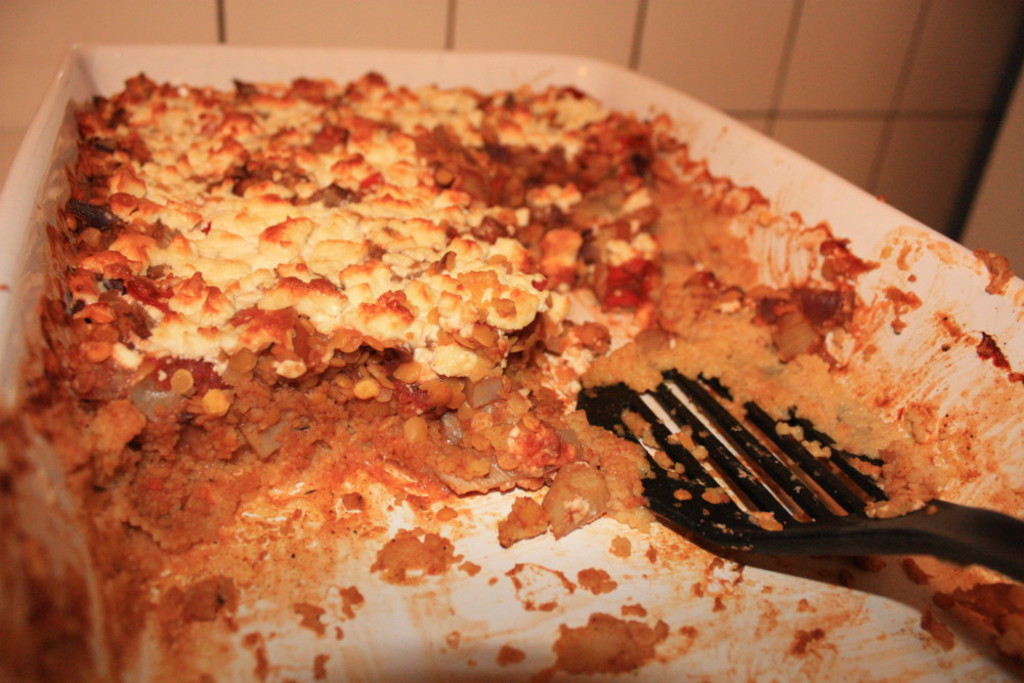
\includegraphics[width=\textwidth]{{Couscous-Auflauf/IMG_6094_small.jpg}}
\end{center}
\vfill
\mbox{ }
\newpage
